\documentclass[
% -- opções da classe memoir --
article,			% indica que é um artigo acadêmico
12pt,				% tamanho da fonte
oneside,			% para impressão apenas no recto. Oposto a twoside
a4paper,			% tamanho do papel. 
english,			% idioma adicional para hifenização
brazil,				% o último idioma é o principal do documento
sumario=tradicional
]{abntex2}
% ---
% PACOTES
% ---
\usepackage{lmodern} % Usa a fonte Latin Modern
\usepackage[T1]{fontenc}% Selecao de codigos de fonte.
\usepackage[utf8]{inputenc}% Codificacao do documento (conversão automática dos acentos)
\usepackage{indentfirst}% Indenta o primeiro parágrafo de cada seção.
\usepackage{nomencl} % Lista de simbolos
\usepackage{color}% Controle das cores
\usepackage{graphicx}% Inclusão de gráficos
\usepackage{microtype}% para melhorias de justificação
\usepackage{gensymb}
\usepackage{caption}
\usepackage{booktabs}

% ---
% Pacotes adicionais, usados apenas no âmbito do Modelo Canônico do abnteX2
% ---
% ---
% Pacotes de citações
% ---
\usepackage[brazilian,hyperpageref]{backref}	 % Paginas com as citações na bibl
%\usepackage[alf,abnt-emphasize=bf]{abntex2cite}	% Citações padrão ABNT
\usepackage[num,overcite,abnt-emphasize=bf]{abntex2cite}	% Citações padrão ABNT
%\citebrackets()
\citebrackets[]
% ---

% ---
% Configurações do pacote backref
% Usado sem a opção hyperpageref de backref
\renewcommand{\backrefpagesname}{Citado na(s) página(s):~}
% Texto padrão antes do número das páginas
\renewcommand{\backref}{}
% Define os textos da citação
\renewcommand*{\backrefalt}[4]{
  \ifcase #1 %
    Nenhuma citação no texto.%
    \or
    Citado na página #2.%
  \else
    Citado nas páginas #2.%
\fi}%
% ---

\graphicspath{{./images/} {/home/victor/Pictures/latex/}}

% --- Informações de dados para CAPA e FOLHA DE ROSTO ---
\titulo{\bfseries Sistemas Embarcados e suas aplicações na agricultura IOT: revisão bibliográfica}
\tituloestrangeiro{Embedded Systems and their applications in agriculture IOT: bibliographic review}

%\autor{Victor Emanuel Almeida}
\autor{
  %UNIOESTE\thanks{``Universidade Estadual do Oeste do Paraná, Foz do Iguaçu, Brasil.'' \url{http://www.unioeste.br/}} 
  %\\[0.5cm]\\
  Victor Emanuel Almeida\thanks{``Estudante de Ciência da Computação na Universidade Estadual do Oeste do Paraná (UNIOESTE), campus de Foz do Iguaçu-PR, Brasil.''\url{http://www.unioeste.br/}}
}

\local{FOZ DO IGUAÇU}
\data{\today}

\instituicao{%
\par
Universidade do Oeste do Paraná 
\par
UNIOESTE
}
\instituicao{Curso de Ciência da Computação, da Universidade Estadual do Oeste do Paraná (UNIOESTE), Campus Foz do Iguaçu-PR, Brasil}

\preambulo{Escrever Preâmbulo}

\tipotrabalho{Trabalho Acadêmico}
% ---

% ---
% Configurações de aparência do PDF final

% alterando o aspecto da cor azul
\definecolor{blue}{RGB}{41,5,195}

% informações do PDF
\makeatletter
\hypersetup{
  %pagebackref=true,
  pdftitle={\@title}, 
  pdfauthor={\@author},
  pdfsubject={software livre},
  pdfcreator={\@author},
  pdfkeywords={software livre},
  colorlinks=true,% false: boxed links; true: colored links
  linkcolor=black,% color of internal links
  citecolor=blue,% color of links to bibliography
  filecolor=magenta,% color of file links
  urlcolor=blue,
  bookmarksdepth=4
}
\makeatother
% --- 

% ---
% compila o indice
% ---
\makeindex
% ---

% ---
% Altera as margens padrões
% ---
\setlrmarginsandblock{3cm}{2cm}{*}
\setulmarginsandblock{3cm}{2cm}{*}
\checkandfixthelayout
% ---

% --- 
% Espaçamentos entre linhas e parágrafos 
% --- 

% O tamanho do parágrafo é dado por:
\setlength{\parindent}{1.25cm}
%\setlength{\parindent}{1.5\lineheight}

% Controle do espaçamento entre um parágrafo e outro:
%\setlength{\parskip}{0.2cm}  % tente também \onelineskip
\setlength{\parskip}{\onelineskip}

% Espaçamento simples
\SingleSpacing

% ----
% Início do documento
% ----
\begin{document}
%\pagenumbering{roman}
% Seleciona o idioma do documento (conforme pacotes do babel)
%\selectlanguage{english}
\selectlanguage{brazil}

% Retira espaço extra obsoleto entre as frases.
\frenchspacing 

% ----------------------------------------------------------
% ELEMENTOS PRÉ-TEXTUAIS
% ----------------------------------------------------------

%---
%
% Se desejar escrever o artigo em duas colunas, descomente a linha abaixo
% e a linha com o texto ``FIM DE ARTIGO EM DUAS COLUNAS''.
%\twocolumn[    		% INICIO DE ARTIGO EM DUAS COLUNAS
%
%---

% página de titulo principal (obrigatório)
%\imprimircapa
%\begin{center}
\maketitle
%{\centered\maketitle\imprimirlocal\imprimirinstituicao}
%\imprimirtitulo
%\vspace{.5cm}

%\imprimirinstituicao
%\end{center}

% titulo em outro idioma (opcional)

% resumo em português
\begin{resumoumacoluna}
  Escrever resumo

  \textbf{Palavras-chave}: Agricultura, Internet das coisas, Tomada de decisão, Sensoreamento.

  \vspace{\onelineskip}

  \noindent
\end{resumoumacoluna}


% resumo em inglês
\renewcommand{\resumoname}{Abstract}
\begin{resumoumacoluna}
  \begin{otherlanguage*}{english}
    Escrever resumo
    \vspace{\onelineskip}
    \noindent

    \textbf {Keywords}: Agriculture, Internet of things, Decision making, Sensing.
  \end{otherlanguage*}  
\end{resumoumacoluna}

%\cleardoublepage
%\pdfbookmark[0]{\contentsname}{toc}
%\tableofcontents*
%\cleardoublepage
%\listoffigures
%\cleardoublepage
%\listoftables

%]  				% FIM DE ARTIGO EM DUAS COLUNAS
% ---

% ----------------------------------------------------------
% ELEMENTOS TEXTUAIS
% ----------------------------------------------------------
\textual
%\setcounter{page}{1}
%\pagenumbering{arabic}
% ----------------------------------------------------------
% Introdução
% ----------------------------------------------------------
\section{Introdução}

Introduzir o assunto de IOT, terminando com citação

Mostrar a relevância da pesquisa, como verificar o que o mundo tem feito deve nos mostrar as melhores práticas bem como as últimas tecnologias disponíveis.

\section{Conceitos e características (Mudar nome)}\label{Conceitos Importantes}
Antes de abordar as principais tecnologias, bem como os principais e mais atuais estudos relacionados a IOT, faz-se necessário elucidar alguns pontos.
\subsection{O que é IOT}\label{O que é IOT}

\subsection{As camadas do IOT}\label{As camadas do IOT}

  Estrutura do IOT: baseada em três camadas\cite{5}
    \begin{enumerate}
      \item A de percepção que seria uma camada de sensores, hardware, que obtém-se dados relevantes a respeito dos fenômenos meteorológicos tais como clima, temperatura do solo, umidade do ar, entre outros.
      \item A camada de comunicação, camada a qual é responsável por enviar os dados coletados pela camada de percepção supracitada para servidores ou aplicações na nuvem, de forma geral para algum tipo de armazenamento. Possuindo diversos protocolos de comunicação tais como \textbf{Ipv4} e \textbf{Ipv6}\cite{camada2}.
      \item A de aplicação, camada a qual trás sentido aos dados coletados pelos sensores, pois é nesse momento que ocorre o processamento dos dados, nessa revisão bibliográfica essa camada será responsável principalmente por mostrar ao agricultor informações relevantes de forma simples e compreensível, bem como informá-lo qual o melhor momento para plantar\cite{1}, ou em quais lugares da plantação tem doenças\cite{2}.
    \end{enumerate}

\section{Materiais e Métodos}\label{Materiais e Métodos}
Perguntar


\begin{table}[!htb]
  \centering
  \caption{Palavras chaves que se repetem}
  \begin{tabular}{|c|l|}
    \hline
    \textbf{Ocorrências} & \textbf{Palavra(s) chave} \\ \hline
    4                    & wireless sensor           \\ \hline
    4                    & precision agriculture     \\ \hline
    4                    & internet of things        \\ \hline
    4                    & sensor network            \\ \hline
    2                    & soil moisture             \\ \hline
    2                    & precision viticulture     \\ \hline
  \end{tabular}
\end{table}

\begin{table}[!htb]
  \centering
  \caption{Ano de publicação dos artigos Qualis A}
  \begin{tabular}{|c|c|}
    \hline
    \textbf{Ano de publicação} & \textbf{Quantidade de artigos} \\ \hline
    2008 & 1 \\ \hline
    2014 & 1 \\ \hline
    2015 & 2 \\ \hline
    2016 & 1 \\ \hline
    2017 & 4 \\ \hline
    2018 & 1 \\ \hline
    2019 & 3 \\ \hline
  \end{tabular}
\end{table}

\begin{figure}[!htb]
  \centering
  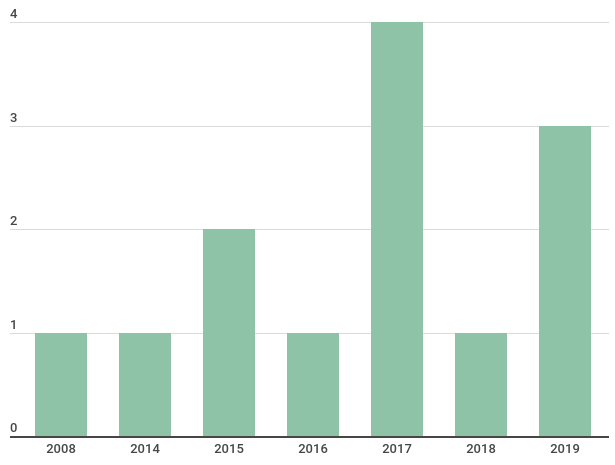
\includegraphics[width=\textwidth]{artigosA.png}
  \caption{\label{fig:artigosA.png}Ano de publicação dos artigos Qualis A}
\end{figure}

\begin{figure}[!htb]
  \centering
  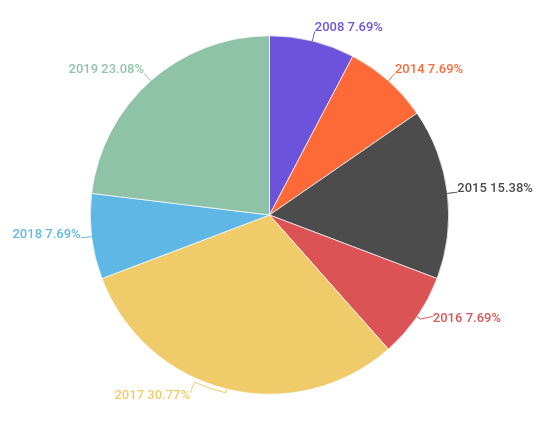
\includegraphics[width=\textwidth]{artigosA_pizza.png}
  \caption{\label{fig:artigosA_pizza.png}Ano de publicação dos artigos Qualis A}
\end{figure}


\section{Sensoreamento (camada de percepção)}\label{Sensoreamento do solo (camada de percepção)}

Tendo em vista a vasta variabilidade dos sensores utilizados nas diversas pesquisas apresentadas, agregamos os melhores resultados a cerca dos sensores.

\subsection{Umidade do solo}\label{Umidade do solo}

\section{Rede (camada de comunicação)}\label{Rede (camada de comunicação)}

\section{Plataformas de tomada de decisão (camada de aplicação)}\label{Plataformas de tomada de decisão}%artigos 1 e 2
Em relação às plataformas de tomada de decisão segundo a pesquisa de~\citeauthor{1} até onde sabe-se no ano de~\citeyear{1} não havia nenhuma plataforma ou \textit{framework} que baseando-se na temperatura do solo fornecesse dados dinâmicos para informar em tempo real decisões agronômicas dependentes do solo, tal como momento do plantio, irrigação entre outros.

Considerando essa lacuna do conhecimento, desenvolveu-se uma ferramenta de suporte à decisão da temperatura do solo, ``\textit{temperature decision support tool}'', seguindo uma metodologia de cinco passos:
\begin{enumerate}
  \item Comparação dos dados climáticos e ambientais, conseguindo a variabilidade em larga escala da temperatura do solo.

  \item Comparação das temperaturas médias em séries históricas.
  \item Comparar variáveis preditoras de clima com as medições realizadas, obtendo previsões.
  \item Transformar o sistema para funcionar em tempo real.
  \item Investigações a longo prazo.
\end{enumerate}

Com o objetivo de aumentar a precisão utiliza-se nove variáveis preditoras de clima, sendo elas: temperatura máxima, radiação diária, diferença entre temperatura máxima e mínima, taxa pluviométrica, latitude, elevação, conteúdo de água do solo, difusão térmica do solo, dia do ano.

Este sistema foi desenvolvido em Shiny (R), e possui uma alta taxa de predição de 92\% de validação cruzada R$_{2}$, RMSE = 1,91, tendência percentual = $-$ 0,01.
Com essas taxas de predição pode-se auxiliar os agricultores de algodão a realizarem o plantio no momento certo, classificando o solo como ``bom'' após três dias com temperaturas acima de 14\textdegree C, dessa maneira após utilizar dados de variáveis preditoras supracitadas recomenda-se ou não o plantio.

Outro sistema de apoio à decisão desenvolvido por~\citeauthor{2}, com o objetivo de monitorar vinhedos para encontrar e tratar ``míldio'' (mofo).
O míldio é uma doença fúngica causada pela \textit{plasmopara viticola oomycete}, doença essa que causa muito prejuízo nas vinícolas\cite{2}. Doença essa muito estudada, sendo assim nessa pesquisa baseando-se nos modelos já existentes de detecção a acompanhamento do fungo, buscou-se a automatização dos mesmos.

O principal modelo utilizado para descobrir qual o momento mais propício de aparecimento do míldio foi o de Goidanich\cite{detectando_milidio}, também chamado de ``regra dos três dez'' pois quando a temperatura média ultrapassa 10\textdegree C, a germinação ultrapassa os 10 cm e o volume de chuva superior a 10 mm, este é o momento propício para uma primeira contaminação da vinha.
Sabendo desses dados expostos por Goidanich\cite{detectando_milidio} percebe-se a necessidade de monitorar três fenômenos, sendo eles: temperatura, umidade e índice pluviométrico, sendo assim precisando de três sensores.

Para desenvolver essa plataforma o autor utilizou o sistema ``\textit{Sense Our Environment}'' (SEnviro), uma plataforma que utilizando-se de software e hardware livres visa baixar o custo e aumentar a eficiência energética dos sensores\cite{2}. O SEnviro contém suas funcionalidades melhor explicado em outra pesquisa\cite{SEnviro} e como já citado nessa seção possui todos os códigos fonte disponível ao público no github\cite{SEnviro_Github}.


Com a estação concluída iniciou-se os testes, detectando em 96,9\% de maneira precisa em que houve o alerta de infecções. Através disso, os agricultores puderam aplicar o tratamento de controle de praga apenas quando necessário, reduzindo assim a quantidade de produtos químicos no solo, a quantidade de horas gastas para verificação e correção de doenças dentro do vinhedo bem como os custos da plantação.

\section{Considerações Finais}
Portanto, percebe-se a vasta área de aplicação de sistemas embarcados para implementações de fazendas inteligentes, tendo em vista que apenas abordando poucos tópicos tais como Plataformas de tomada de decisão, como citado na seção~\ref{Plataformas de tomada de decisão} e seus sensores, como citado na seção~\ref{Sensoreamento do solo (camada de percepção)}.

Outrossim a partir dos sistemas de previsão tais como\cite{1},\cite{2} auxiliaram produtores agrícolas a terem uma maior eficiência na hora de plantar, colher e obter mais informações a respeito da plantação sem o trabalho de verificar manualmente.

Em relação aos sensores, percebeu-se uma grande variedade tanto em relação a preços precisões entre outros. Dessa forma cada em aplicação deve-se analisar qual a opção mais viável não existindo sensor perfeito para todas as aplicações, mas sim sensor perfeito para uma aplicação específica.

% ----------------------------------------------------------
% ELEMENTOS PÓS-TEXTUAIS
% ----------------------------------------------------------
\postextual

% ----------------------------------------------------------
% Referências bibliográficas
% ----------------------------------------------------------
\cleardoublepage
\bibliography{ref}

% ----------------------------------------------------------
% Glossário
% ----------------------------------------------------------
%
% Há diversas soluções prontas para glossário em LaTeX. 
% Consulte o manual do abnTeX2 para obter sugestões.
%
%\glossary

\end{document}
